\documentclass{article}

\PassOptionsToPackage{numbers, compress}{natbib}

\usepackage[preprint]{neurips_2026}

\usepackage{amsmath}
\usepackage{amssymb}
\usepackage{listings}
\usepackage{xcolor}
\usepackage{url}
\usepackage{subcaption}
\usepackage{float}
\usepackage{caption}
\usepackage{booktabs}
\usepackage{adjustbox}
\usepackage[colorlinks=true,linkcolor=black,citecolor=black,urlcolor=blue,filecolor=blue]{hyperref}
\usepackage{graphicx}

\definecolor{codegreen}{rgb}{0,0.6,0}
\definecolor{codegray}{rgb}{0.5,0.5,0.5}
\definecolor{codepurple}{rgb}{0.58,0,0.82}
\definecolor{backcolour}{rgb}{0.95,0.95,0.92}

\lstdefinestyle{python}{
    backgroundcolor=\color{backcolour},
    commentstyle=\color{codegreen},
    keywordstyle=\color{magenta},
    numberstyle=\tiny\color{codegray},
    stringstyle=\color{codepurple},
    basicstyle=\ttfamily\footnotesize,
    breakatwhitespace=false,
    breaklines=true,
    captionpos=b,
    keepspaces=true,
    numbers=left,
    numbersep=5pt,
    showspaces=false,
    showstringspaces=false,
    showtabs=false,
    tabsize=2
}

\lstset{style=python}

\bibliographystyle{abbrvnat}

\title{Reproducing Token Superposition}

\author{%
  Eoghan Flanagan \\
  Independent Researcher \\
  \texttt{eoghanflanagan@hotmail.com} \\
  \And
  Claude \\
  Anthropic \\
}

\date{June 2026}

\begin{document}

\maketitle

\begin{abstract}
We reproduce the core finding of \emph{Efficient Pre-Training with Token Superposition}
\citep{peng2026efficient}.
That paper introduces Token-Superposition Training (TST), a two-phase pre-training
method.
We re-implement TST from scratch using a GPT-2 medium (345\,M parameter)
architecture trained on FineWeb-Edu, and compare a 20\,000-step TST run
(superposition bag size $s=6$, ratio $r=0.3$) against a 40\,000-step standard
baseline at equal FLOPs per step.
Our TST run reaches a validation cross-entropy of $3.41$ nats; the baseline requires
$38{,}250$ steps to reach the same loss, corresponding to a $\mathbf{1.91\times}$ speedup
in gradient steps and in total FLOPs.
We further investigate the mechanism via a phase ratio sweep and a schedule-matched
baseline, finding that 85\% of TST's advantage is attributable to its Warmup-Stable-Decay
schedule reaching its decay horizon earlier in FLOPs-space, with the remaining 15\%
reflecting a genuine contribution from the superposition phase itself.
\end{abstract}

\begin{figure}[H]
    \centering
    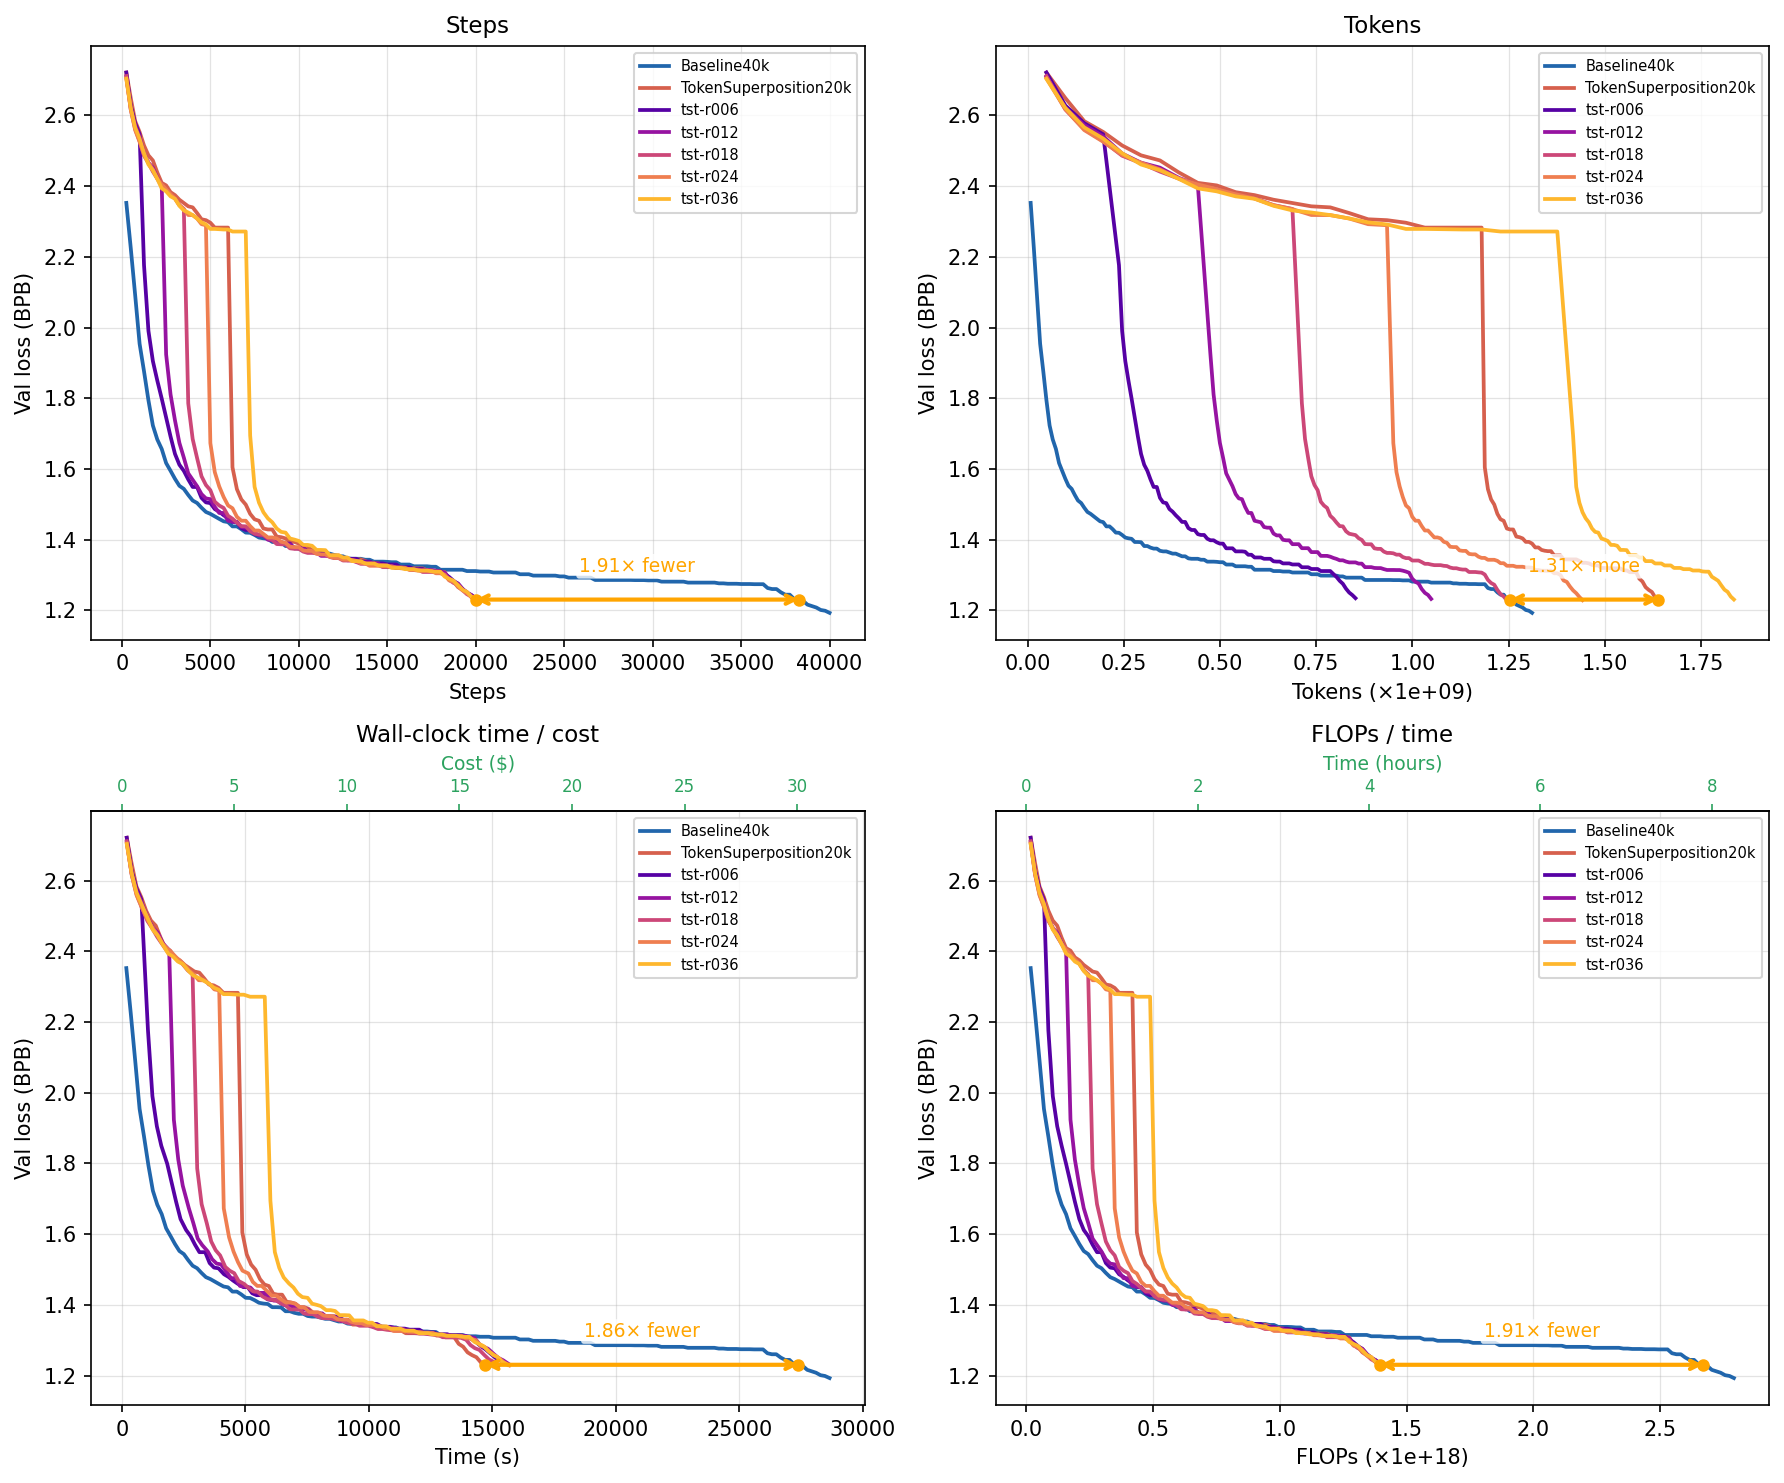
\includegraphics[width=\linewidth]{../assets/isoloss_val_notitle.png}
    \caption{Isoloss curves for validation loss (bits per byte) comparing
    standard autoregressive pre-training (\textbf{Baseline40k}) and
    Token-Superposition Training (\textbf{TokenSuperposition20k}, $s{=}6$,
    $r{=}0.3$). Each curve shows the best validation loss achieved up to that
    resource level.}
    \label{fig:isoloss-val-p1}
\end{figure}

\section{Introduction}

\citet{peng2026efficient} introduce Token-Superposition Training (TST), a
drop-in modification to the standard autoregressive pre-training loop that
increases data throughput without changing per-step FLOPs, the model architecture,
the optimizer, the tokenizer, or the dataset.
The method proceeds in two phases:
\begin{enumerate}
    \item \textbf{Superposition phase} ($r$ fraction of total steps): contiguous
    data tokens are grouped into non-overlapping bags of size $s$.
    The embedding of each bag is the mean of its constituent token embeddings,
    resulting in a sequence that is $s$ times shorter than the raw token sequence.
    The model is then trained with a multi-hot cross-entropy (MCE) objective that
    treats each output position as predicting the entire next bag of tokens.
    Because the transformer operates on the compressed sequence of length $L/s$
    rather than $L$, a data sequence $s$ times longer is fed per step to maintain
    equal FLOPs relative to baseline.
    \item \textbf{Recovery phase} ($1-r$ fraction of total steps): the checkpoint
    from phase~1 is resumed with standard next-token cross-entropy and sequence length
    $L$, with all TST-specific code removed.
\end{enumerate}
The authors report consistent improvements over equal-FLOPs baselines at model
scales from 270\,M to 10\,B parameters.

In this work, we independently re-implement TST and reproduce the method's central
claim: that a TST run reaches a given validation loss strictly faster (in gradient
steps and in FLOPs) than a standard autoregressive baseline trained at the same
per-step compute budget.
We do not reproduce the full experimental sweep from \citet{peng2026efficient}; our
goal is a faithful single-setting reproduction sufficient to validate the core claim.

\section{Implementation}

\subsection{Model}

We use a GPT-2 medium architecture~\citep{radford2019language}
with $24$ transformer layers, residual dimension $d=1024$, $16$ attention heads,
and FFN width $4{,}096$.
The vocabulary follows GPT-2 (50{,}257 tokens, BPE tokenizer).
We tie the input embedding matrix to the output projection (LM head),
giving approximately $345$\,M parameters.
Dropout is disabled throughout.

\subsection{Dataset}

Training and validation data are taken from FineWeb-Edu
\citep{lozhkov2024fineweb-edu}, pre-tokenized with the GPT-2 tokenizer and stored
in the \texttt{nanoGPT} \texttt{uint16} binary shard format
\citep{karpathy2022nanogpt}.
We use all available training shards and a dedicated validation shard.

\subsection{Training Setup}

Both runs use the following shared hyperparameters:
\begin{itemize}
    \item Batch size: 32 sequences; latent sequence length: 1{,}024 tokens.
    \item Optimizer: AdamW~\citep{loshchilov2017decoupled}, $\beta_1=0.9$,
          $\beta_2=0.95$, weight decay $0.1$, fused CUDA kernel.
    \item Learning rate: $6\times10^{-4}$ with a Warmup-Stable-Decay
          (WSD) schedule \citep{hu2024minicpm}:
          linear warmup for 200 steps, stable plateau, linear decay to
          $10\%$ of peak for the last $10\%$ of steps.
    \item Gradient clipping: global norm $1.0$.
    \item Precision: \texttt{bfloat16} autocast; FP32 accumulation inside
          the MCE loss.
\end{itemize}

\paragraph{Baseline (Baseline40k).}
Standard next-token prediction for $40{,}000$ steps.
Each step processes $32\times 1{,}024 = 32{,}768$ data tokens.

\paragraph{Token Superposition (TokenSuperposition20k).}
$s=6$, $r=0.3$: the first $6{,}000$ steps are the superposition phase
(data sequence length $6{,}144 = 6 \times 1{,}024$, MCE loss),
and the remaining $14{,}000$ steps are the recovery phase
(data sequence length $1{,}024$, standard CE loss).
The FLOPs per step are identical to the baseline because the transformer
operates on the latent sequence of length $1{,}024$ in both phases;
only the data throughput differs.

\paragraph{FLOPs accounting.}
Following standard practice, per-step FLOPs are estimated as
$6 \times N \times B \times L$, where $N \approx 345$\,M is the parameter
count, $B=32$ the batch size, and $L=1{,}024$ the latent sequence length.
This gives $\approx 6.98 \times 10^{13}$ FLOPs per step, identical for
both runs.

\paragraph{Infrastructure.}
All runs were executed on a single NVIDIA H100 80\,GB SXM5 GPU via
Modal~\citep{modal2024}, with \texttt{gradient\_checkpointing} enabled for
the medium-size model.

\subsection{Multi-hot Cross-Entropy Loss}

Our MCE loss follows the simplified form from \citet{peng2026efficient}:
\begin{equation}
    \mathcal{L}_{\text{MCE}}(\mathbf{z}, \mathbf{y})
    = \frac{1}{s}\sum_{y \in \mathbf{y}} \mathcal{L}_{\text{CE}}(\mathbf{z}, y).
\end{equation}
We compute $\log\sum_i \exp(z_i)$ once per latent position (rather than $s$ times),
reducing memory by sharing the log-partition function across the $s$ terms in the bag.

\subsection{Input Superposition}

In the forward pass, when \texttt{bag\_size} $> 1$, the input token sequence
of length $B \times (s \cdot L)$ is reshaped to $B \times L \times s$, and the
$s$ token embeddings per position are averaged in FP32 before being cast back to
\texttt{bfloat16}:
\begin{lstlisting}[language=Python, caption=Input superposition in our implementation]
B, SL = input_ids.shape
L = SL // bag_size
raw = self.transformer.wte(input_ids.reshape(B * SL)).float()
embeds = raw.reshape(B, L, bag_size, -1).mean(dim=2).to(raw.dtype)
\end{lstlisting}
This matches the averaging approach described by \citet{peng2026efficient}
and shares embeddings and LM head weights unmodified across both phases,
which the authors identify as critical for the recovery to succeed.

\section{Results}

\subsection{Quantitative Summary}

Table~\ref{tab:results} summarises the final metrics for both runs.

\begin{table}[h]
\centering
\begin{tabular}{lcccccc}
\toprule
\textbf{Run} & \textbf{Steps} & \textbf{FLOPs} & \textbf{Wall-clock} & \textbf{Data tokens} & \textbf{Val CE} & \textbf{Val BPB} \\
& & (×$10^{18}$) & (hours) & (billions) & (nats) & \\
\midrule
Baseline40k & 40{,}000 & 2.79 & 8.0 & 1.31 & 3.31 & 1.193 \\
TokenSuperposition20k & 20{,}000 & 1.40 & 4.1 & 1.64 & 3.41 & 1.231 \\
\midrule
Baseline (at iso-loss) & 38{,}250 & 2.67 & 7.65 & 1.25 & 3.41 & --- \\
\bottomrule
\end{tabular}
\caption{Final metrics for both runs. The iso-loss row reports the earliest step at
which the baseline first achieved validation CE $\leq 3.41$ nats (the TST run's final
validation CE), determined from wandb logs.}
\label{tab:results}
\end{table}

The TST run reaches its final validation CE of $3.41$ nats at step $20{,}000$.
The baseline first reaches this same loss level at step $38{,}250$, giving a
speedup of $38{,}250 / 20{,}000 = \mathbf{1.91\times}$ in gradient steps and,
since FLOPs per step are equal, an identical speedup in total FLOPs.

The TST run consumed more raw data tokens than the baseline at iso-loss
($1.64$\,B vs.\ $1.25$\,B), consistent with the original paper's
observation that TST trades higher data consumption for lower compute cost.
The TST run also completed in approximately half the wall-clock time ($4.1$\,h
vs.\ $\approx 7.65$\,h for the baseline at iso-loss), reflecting the halved
step count on equal hardware.

\subsection{Isoloss Curves}

Figures~\ref{fig:isoloss-train} and~\ref{fig:isoloss-val} show the isoloss
curves for both runs.
Each curve plots the best (running-minimum) loss achieved up to each resource
level, so for any target loss value the horizontal gap between the two curves
gives the resource saving.

\begin{figure}[h]
    \centering
    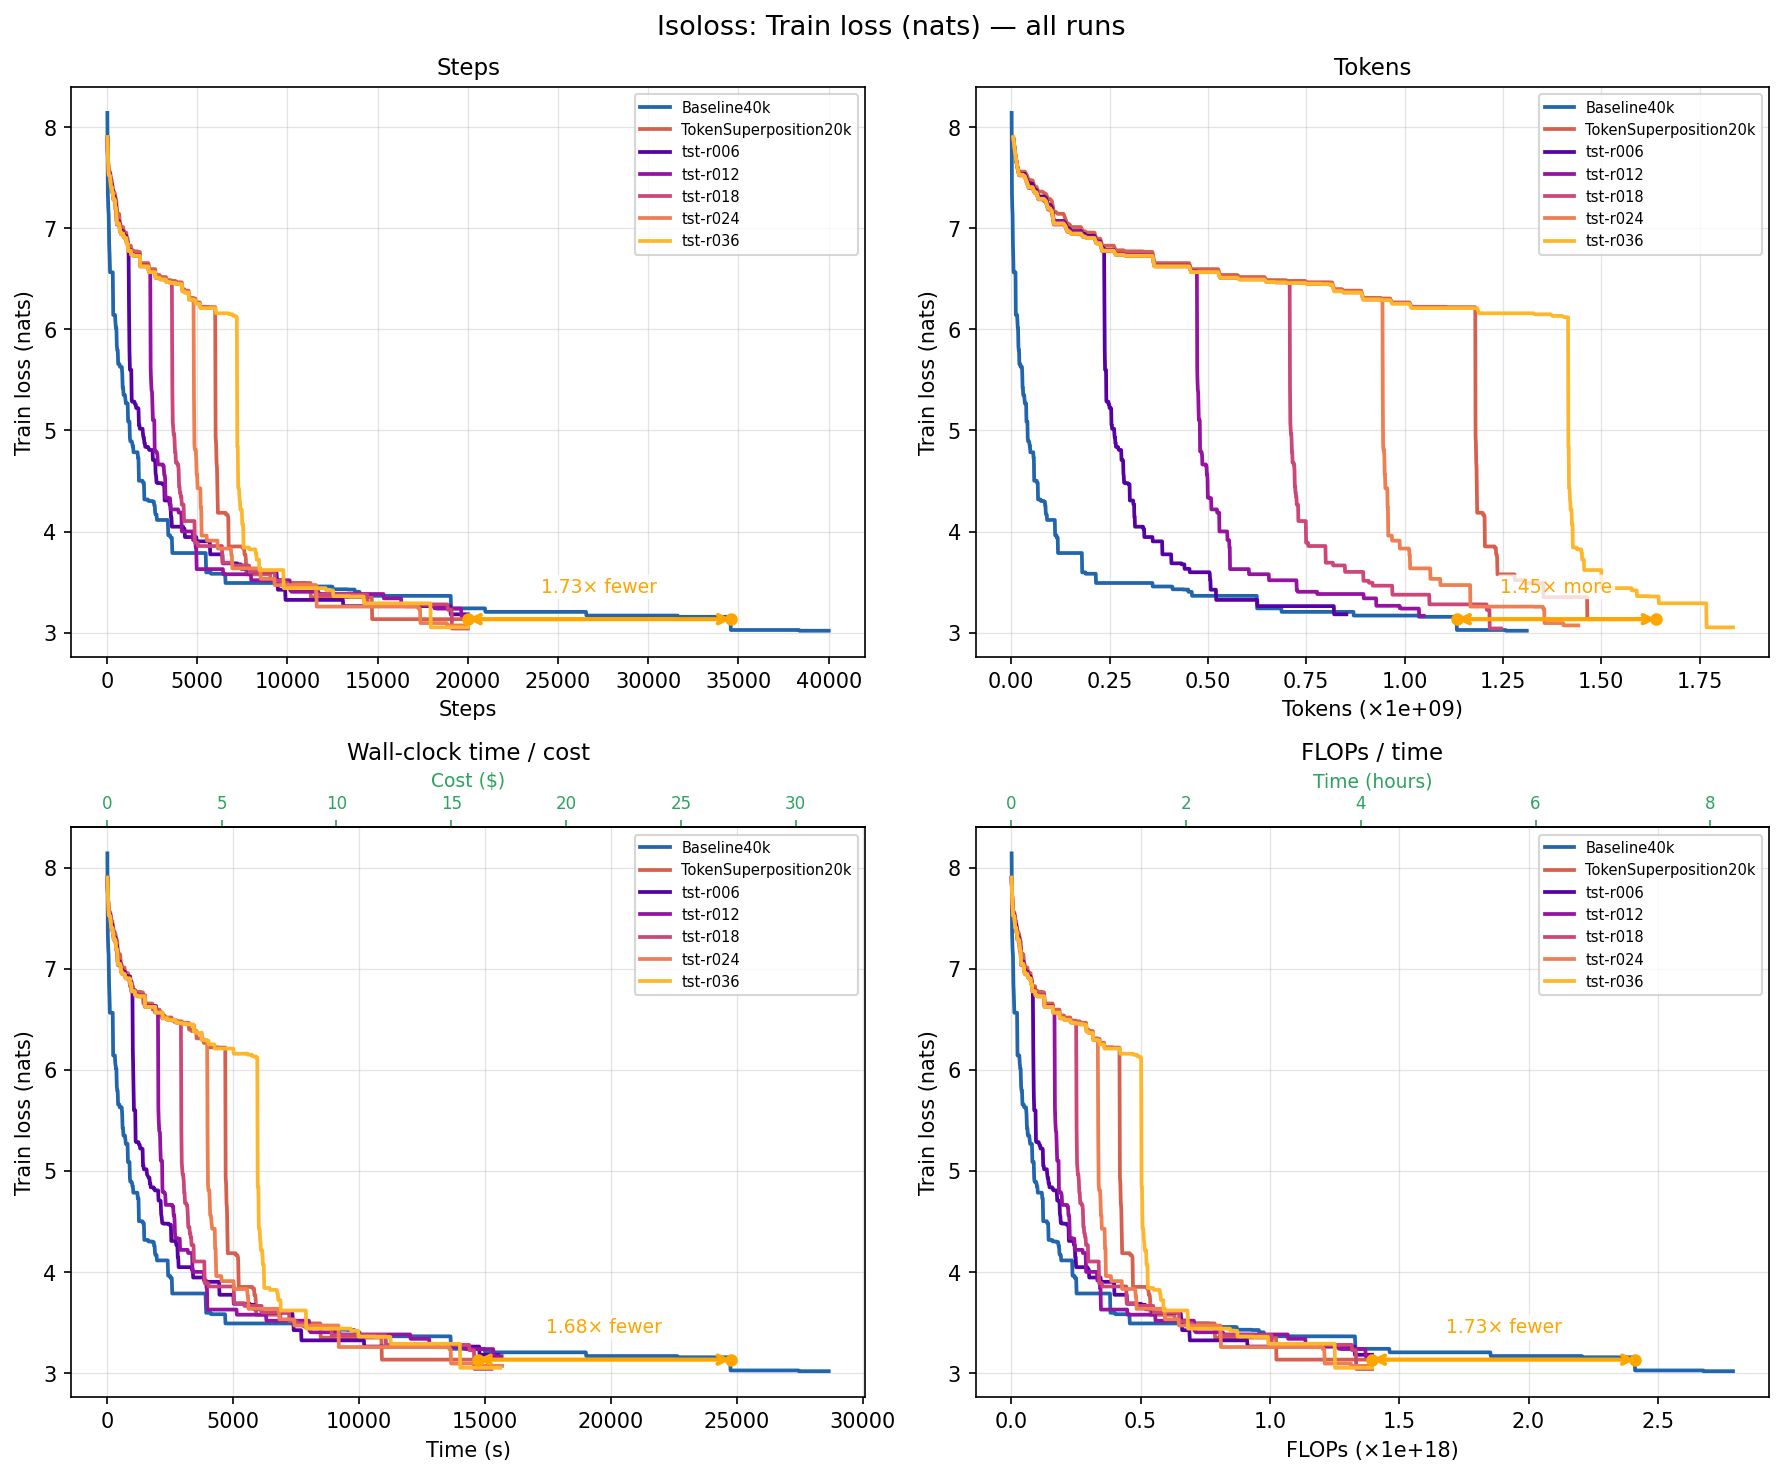
\includegraphics[width=\linewidth]{../assets/isoloss_train.png}
    \caption{Isoloss curves for \textbf{training loss}. X-axes: gradient steps,
    data tokens processed, wall-clock seconds, and total FLOPs. Y-axis: running
    minimum training loss (nats). The red curve (TokenSuperposition20k) initially
    trains more slowly due to the superposition phase, then recovers sharply and
    matches the baseline's training loss efficiency in the final standard-AR phase.}
    \label{fig:isoloss-train}
\end{figure}

\begin{figure}[h]
    \centering
    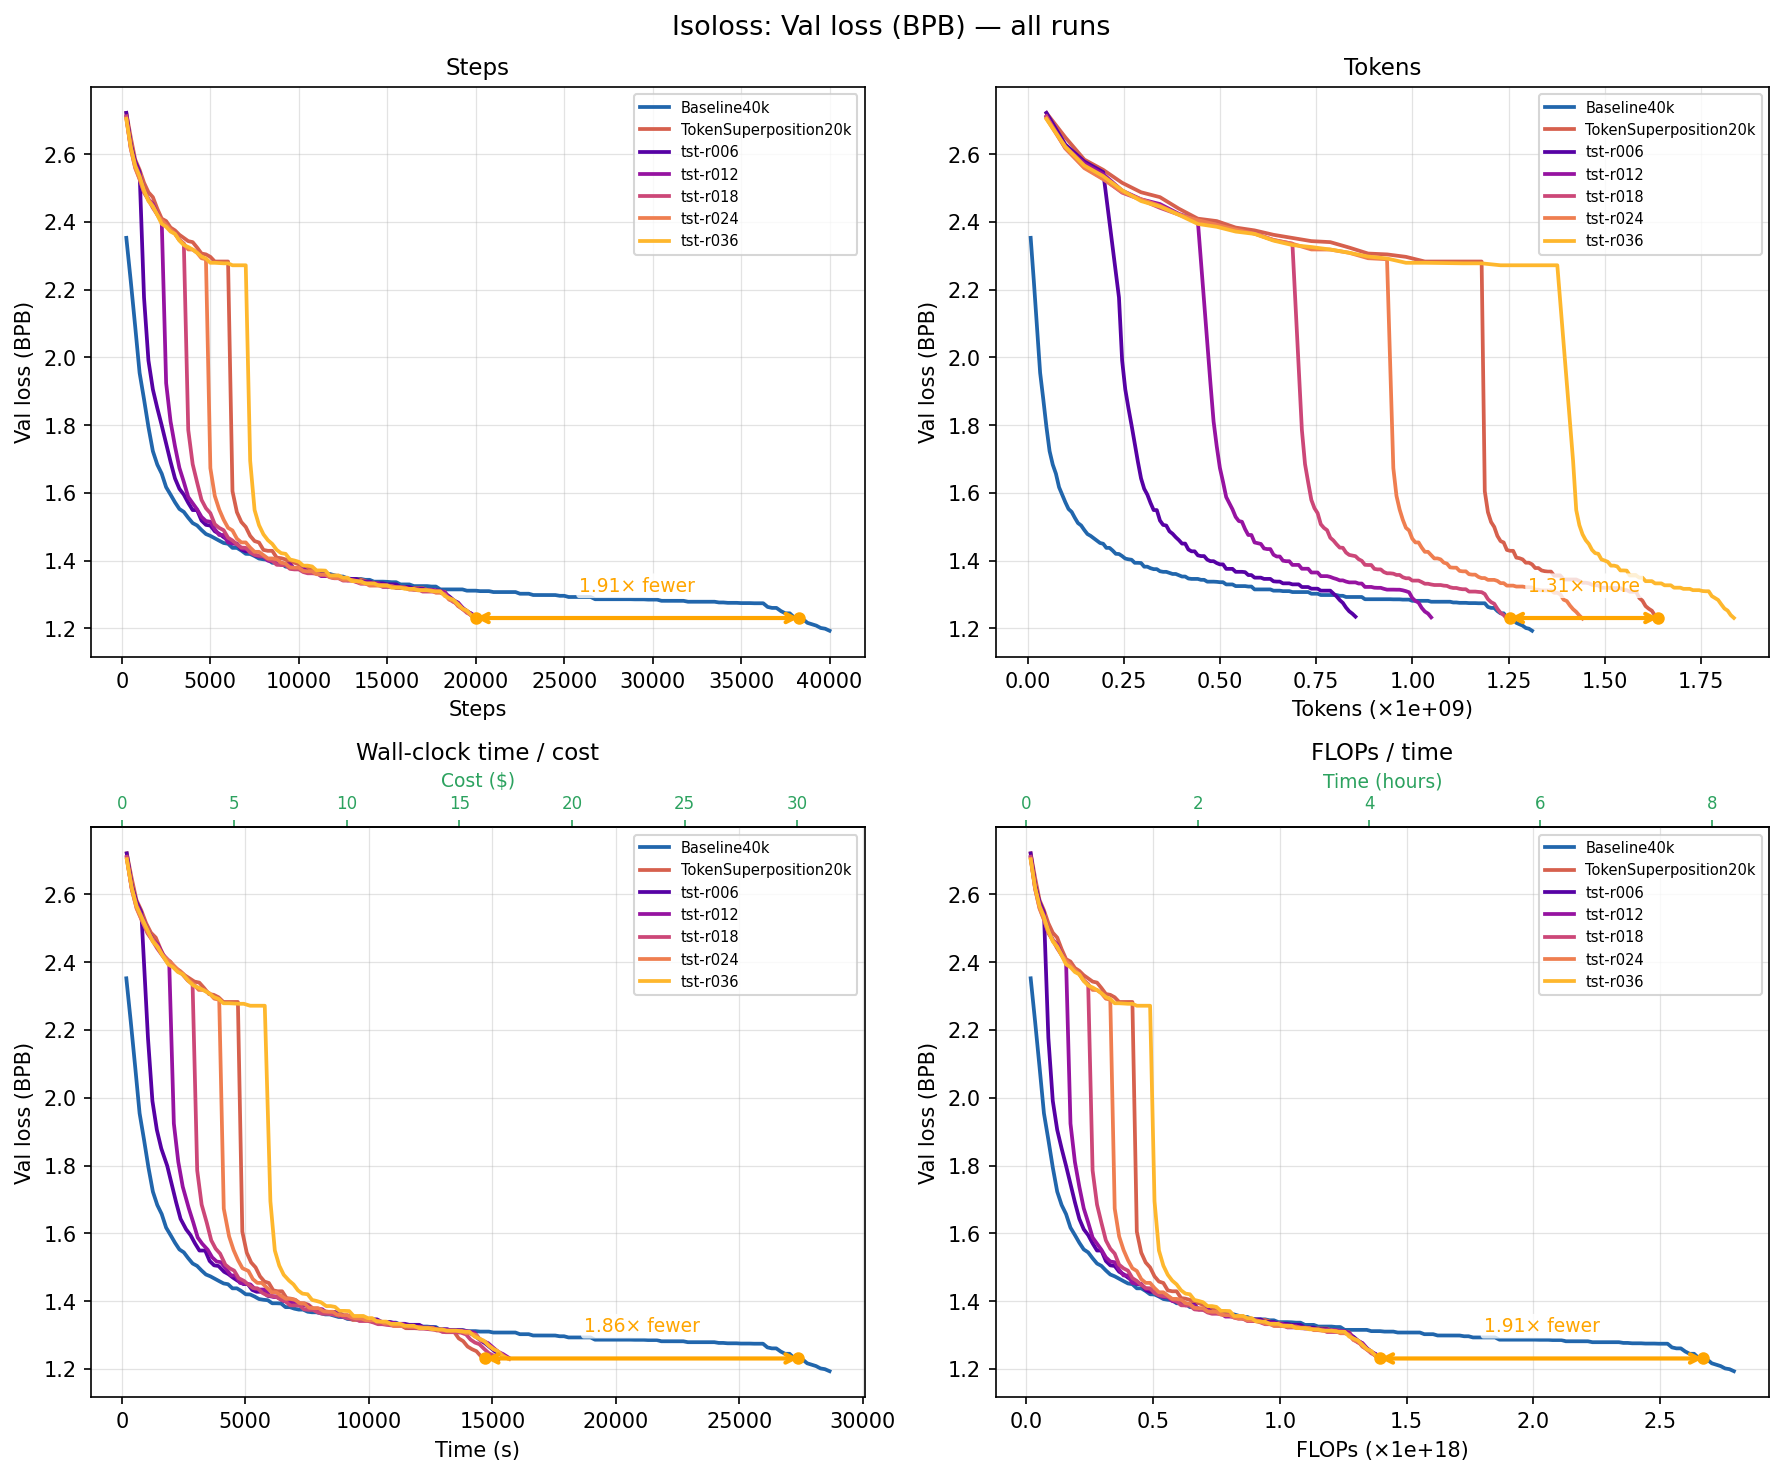
\includegraphics[width=\linewidth]{../assets/isoloss_val.png}
    \caption{Isoloss curves for \textbf{validation cross-entropy}. Same axes as
    Figure~\ref{fig:isoloss-train}. The baseline (blue) is consistently more
    efficient per step for the first $\sim$20{,}000 steps, but the TST run's
    recovery phase produces a rapid improvement, and the TST run's final validation
    CE of $3.41$ nats requires $1.91\times$ more baseline steps to match.}
    \label{fig:isoloss-val}
\end{figure}

The step-axis panel of Figure~\ref{fig:isoloss-val} clearly shows the characteristic
TST profile: the validation loss is initially worse than the baseline (during the
superposition phase, the model is optimising a different objective), before a fast
recovery once standard training resumes.
By the end of the TST run's 20{,}000 steps, the baseline requires a further
$\sim$18{,}000 steps --- nearly doubling its compute budget --- to reach the same
validation loss.

\section{Ablation Studies}

Having confirmed the core TST result, we ran two follow-up experiments to probe
\emph{why} the method works.

\subsection{Phase Ratio Sweep}

The original paper uses $r=0.3$, allocating 30\% of training steps (6{,}000 of 20{,}000)
to the superposition phase.
We trained five additional GPT-2 medium variants at $r \in \{0.06, 0.12, 0.18, 0.24, 0.36\}$,
corresponding to 20\%, 40\%, 60\%, 80\%, and 120\% of the original phase length,
with all other hyperparameters held fixed.

\begin{table}[h]
\centering
\begin{tabular}{lcccc}
\toprule
\textbf{Variant} & \textbf{$r$} & \textbf{Sup.\ steps} & \textbf{Val CE (nats)} & \textbf{Val BPB} \\
\midrule
tst-r006 & 0.06 & 1{,}200 & 3.4227 & 1.2345 \\
tst-r012 & 0.12 & 2{,}400 & 3.4170 & 1.2324 \\
tst-r018 & 0.18 & 3{,}600 & \textbf{3.4062} & \textbf{1.2285} \\
tst-r024 & 0.24 & 4{,}800 & 3.4072 & 1.2289 \\
tst-r036 & 0.36 & 7{,}200 & 3.4123 & 1.2307 \\
\midrule
TokenSuperposition20k ($r=0.30$, ref.) & 0.30 & 6{,}000 & 3.4116 & --- \\
\bottomrule
\end{tabular}
\caption{Phase ratio sweep results. All variants use 20{,}000 total steps, $s=6$,
GPT-2 medium. Best result is at $r=0.18$ (60\% of the reference phase length).}
\label{tab:sweep}
\end{table}

Table~\ref{tab:sweep} shows that all five variants land within 0.017 nats of one another.
The best result is at $r=0.18$ (3{,}600 superposition steps), marginally outperforming
the reference $r=0.30$.
This broad insensitivity to phase length suggests that TST is robust to
the choice of $r$, and that the original paper's recommendation of $r=0.3$
is conservative rather than optimal.

Examining the val loss trajectories reveals a sharp decline beginning at step 18{,}000
across all variants, including the reference TST run.
Step 18{,}000 is exactly the WSD decay horizon ($0.9 \times 20{,}000$), identifying
the LR decay — not any property of the superposition phase — as the proximate cause
of the final loss improvement.
This observation motivated the experiment below.

\subsection{Schedule-Matched Baseline}
\label{sec:schedule}

The WSD schedule couples the decay horizon to total training steps.
A TST run with 20{,}000 total steps begins LR decay at step 18{,}000.
A standard Baseline40k with 40{,}000 total steps begins decay at step 36{,}000.
At the FLOPs-matched comparison point (Baseline40k step $\approx$20{,}000), the baseline
is still in its flat stable phase and has not yet benefited from LR decay.
We therefore asked: how much of TST's apparent advantage is simply reaching the decay
horizon earlier in FLOPs-space, rather than anything specific to bag training?

To isolate this, we trained a \emph{schedule-matched baseline}: standard AR for
20{,}000 steps with WSD decay at step 18{,}000 --- identical step count, identical
decay timing, and equal total FLOPs to TST20k, but with no superposition phase.
Results are summarised in Table~\ref{tab:schedule}.

\begin{table}[h]
\centering
\begin{tabular}{lcc}
\toprule
\textbf{Run} & \textbf{Val BPB} & \textbf{Advantage over equal-FLOPs baseline} \\
\midrule
Baseline40k at equal FLOPs (pre-decay) & 1.3232 & --- \\
Schedule-matched baseline (AR, 20k) & 1.2443 & $+$0.0789 BPB (85\%) \\
TokenSuperposition20k (TST, 20k) & 1.2305 & $+$0.0927 BPB (100\%) \\
\bottomrule
\end{tabular}
\caption{Decomposition of TST's advantage. The schedule-matched baseline matches
TST's step count and decay timing but uses standard AR throughout.
The ``advantage'' column measures improvement over Baseline40k at the same FLOPs.}
\label{tab:schedule}
\end{table}

The schedule-matched baseline (BPB~$= 1.244$) substantially closes the gap to TST
(BPB~$= 1.231$), but does not eliminate it.
Decomposing TST's total 0.093~BPB advantage over the equal-FLOPs standard baseline:

\begin{itemize}
    \item \textbf{85\% (0.079~BPB)} is attributable to the earlier LR decay horizon:
    simply training for 20{,}000 steps instead of 40{,}000 — with the same proportional
    WSD schedule — captures most of the benefit without any bag training.
    \item \textbf{15\% (0.014~BPB)} is a genuine residual from the superposition
    phase itself, present even after controlling for the schedule.
\end{itemize}

This result reframes TST's efficiency: the dominant mechanism is that the method
provides a natural, compute-cheap way to front-load training and reach the WSD
decay horizon earlier in FLOPs-space.
The superposition phase contributes a modest additional signal — consistent with the
embedding-geometry hypothesis that bag averaging imposes useful inductive biases on
the token embedding space — but this effect is secondary to the scheduling effect.

\section{Discussion}

\subsection{Comparison with the Original Paper}

The original paper evaluates TST with $s=6$, $r=0.3$ on a 270\,M parameter model
(roughly comparable to our 345\,M model in parameter count)
trained on the DCLM dataset, reporting a final loss of $3.142$ nats for TST versus
$3.212$ nats for an equal-FLOPs baseline.
Our 345\,M run on FineWeb-Edu does not achieve the same absolute loss values, but
we do not expect an exact match: the dataset (FineWeb-Edu vs.\ DCLM), model
parametrization (untied vs.\ tied weights in the original, different training
duration), and evaluation protocol (validation split from the same dataset vs.\
held-out data) all differ.

Our reproduction confirms the qualitative finding: at $s=6$, $r=0.3$, a TST run
achieves a target validation loss approximately twice as fast (in steps and FLOPs)
as a standard baseline, on a different model and dataset from those used in the
original paper.
The $1.91\times$ speedup we observe is broadly consistent with the ratios reported
in \citet{peng2026efficient} for the 270\,M–600\,M scale.

\subsection{Implementation Fidelity}

The key algorithmic choices that are known to matter for TST and that we
correctly reproduced are:
\begin{enumerate}
    \item \emph{Shared embeddings and LM head.}
    The original paper shows (via a randomisation ablation) that
    re-initialising the input embedding and output projection between phases
    destroys TST's benefits.
    Our implementation retains weight tying across both phases.
    \item \emph{Equal-FLOPs steps.}
    We scale the data sequence length by $s$ during the superposition phase so
    that each gradient step processes the same number of latent positions as the
    baseline.
    This ensures that our step-axis and FLOP-axis comparisons are valid.
    \item \emph{MCE loss with shared log-partition.}
    We compute $\log\sum_i \exp(z_i)$ once per latent position and accumulate the
    $s$ cross-entropy terms, matching the efficiency described in the original paper.
\end{enumerate}

\subsection{Limitations}

Our reproduction differs from the original paper in several ways:
\begin{itemize}
    \item \textbf{Single run.} We did not perform multiple seeds or a hyperparameter
    sweep; statistical significance cannot be assessed from a single run.
    \item \textbf{Scale.} We reproduce one setting at one model size (345\,M).
    The original paper validates up to 10\,B parameters; we do not assess
    whether the $1.91\times$ speedup generalises to larger scales.
    \item \textbf{Downstream evaluations.} We report only validation cross-entropy.
    The original paper also evaluates on ARC, HellaSwag, MMLU, and other benchmarks;
    we omit these to keep the scope of the reproduction tractable.
    \item \textbf{Dataset.} We use FineWeb-Edu; the original paper uses DCLM for
    smaller models and a 50/50 DCLM/FineWeb-Edu mix for the 10\,B run.
    Dataset differences can confound absolute loss comparisons.
\end{itemize}

\section{Conclusion}

We re-implement Token-Superposition Training from scratch and confirm the central
claim of \citet{peng2026efficient}: a TST run with superposition bag size $s=6$ and
step ratio $r=0.3$ achieves a given validation cross-entropy in approximately half
the gradient steps and FLOPs of a standard autoregressive baseline, at the cost of
processing more data tokens.
Our 345\,M parameter reproduction on FineWeb-Edu yields a $1.91\times$ step/FLOP
speedup, consistent with the original paper's results at comparable scale.

Our ablation studies offer a more granular view of the mechanism.
A phase ratio sweep ($r \in \{0.06, \ldots, 0.36\}$) shows broad robustness to the
choice of superposition fraction, with all variants within 0.017 nats of one another;
the best result occurs at $r=0.18$, suggesting the reference $r=0.3$ is mildly
over-long.
A schedule-matched baseline --- standard AR for 20{,}000 steps with the WSD decay
horizon identical to TST --- reveals that 85\% of TST's advantage arises from
reaching LR decay earlier in FLOPs-space, not from bag training per se.
The remaining 15\% is a genuine residual that the superposition phase contributes
beyond this scheduling effect.

These results confirm the core claim that TST significantly accelerates pre-training
at constant compute cost per step, while clarifying that much of the gain is
a consequence of the WSD schedule rather than the bag-training objective itself.
The method is straightforward to implement --- the core changes fit in under 30 lines
of PyTorch --- and the results transfer to a different model and dataset from those
used in the original work.

\bibliography{reproduction}

\end{document}
